\setlength{\parskip}{1em}

\chapter{Zadání}

MediTabMobile je aplikace pro správu záznamů o pacientech ve fakultní nemocnici na mobilních zařízeních. Doplňuje tabletovou aplikaci MediTab (vývoj David Pivovar, Daniel Švarc) a desktopovou aplikaci WinMedicalc (vývoj Medicalc software s.r.o.).

Aplikace má 2 části, správu ordinovaných léků a bilanci tekutin. Je napsána v jazyce Java, nativním jazyce pro Android.


%%%%%%%%%%%%%%%%%%%%%%%%%%%%%%%%%%%%%%%%%%%%%%%%%%%%%%%%%%%%%%%%%%%%%%%%%%%%%%%%%%%%%%%%%%%%%%%%%%%%

\chapter{Implementace}

Aplikace má 4 aktivity. První pro přihlášení uživatele, druhá zobrazuje výběr pacientů, třetí zobrazuje seznam léků předepsaných pacientovi a bilanci tekutin, a poslední umožňuje zápis podávání léků.

\section{Data}

Data jsou načítána z textových souborů. Soubory jsou z důvodu testování v raw directory. Raw directory ovšem neumožňuje opětovný zápis do souborů. Tato možnost byla zvolena proto, že nedisponuji zařízením s funkčním čtením a ukládáním na SD kartu, a neměl bych jak aplikaci otestovat. Data se načítají ze souboru při volání onCreate() (onCreateView() v případě fragmentů u medikace a bilance tekutin). Při volání onPause() by se měla data uložit.

\section{Přihlášení}

Aktivita s dvěmi textovými poli a buttonem pro přihlášení (obr. \ref{login}). Po kliknutí na button se otestuje shodnost přihlašovacího jména a hesla. Při úspěšném přihlášení se zobrazí aktivita s výberem pacientů. Při neúspěšném přihlášení se objeví Toast informující uživatele.

\begin{figure}[H]
	\centering
	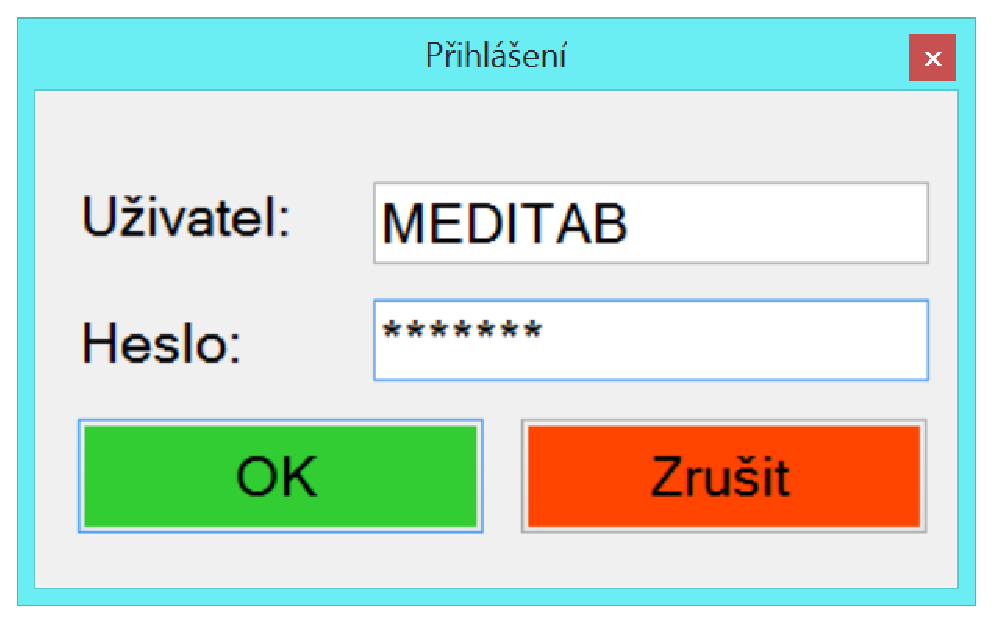
\includegraphics[width=0.4\textwidth]{img/login.eps}
	\caption{Přihlášení}
  \label{login}
\end{figure}



\section{Výběr pacienta}

Seznam pacientů je v ListView (obr. \ref{pacient}. Seznam pacientů a layout (simple\_list\_item\_1) pro ListView zprostředkovává ArrayAdapter z pole se jmény a ID pacienta. Vybráním pacienta se zobrazí aktivita s léky a bilancí tekutin. Aktivitě se předá string s ID pacienta.

\begin{figure}[H]
	\centering
	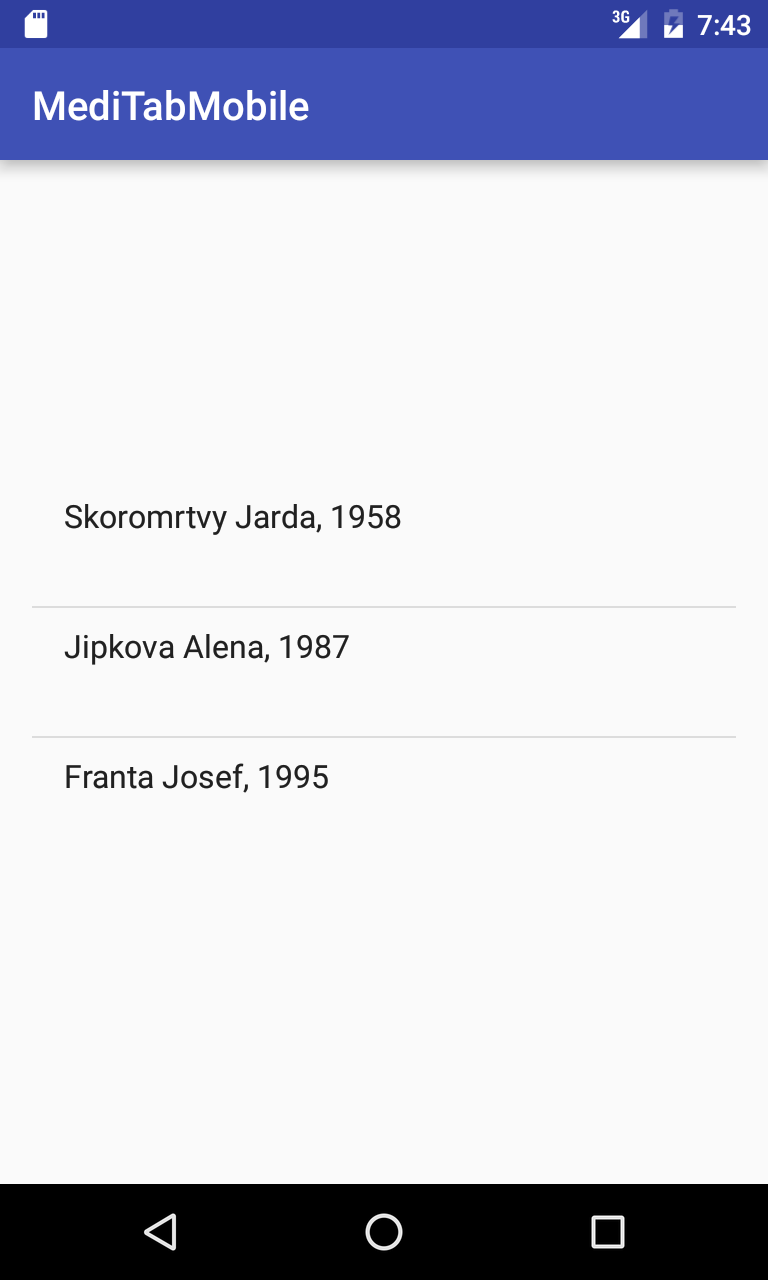
\includegraphics[width=0.4\textwidth]{img/pacient.eps}
	\caption{Výběr pacienta}
  \label{pacient}
\end{figure}

\section{Medikace a bilance tekutin}

Tato aktivita obsahuje 2 View (fragmenty). Přepínání mezi jednotlivými View se provádí pomocí Swipe.

První View zobrazuje předepsané léky pacientovi v ListView (obr. \ref{medikace}). Seznam léků  a layout (simple\_list\_item\_2) pro ListView zprostředkovává ArrayAdapter z pole léků předepsaných danému pacientovi (podle ID pacienta). Vybráním léku se zobrazí aktivita s jednotlivými ordinacemi léku. Aktivitě se předá string s ID pacienta a string s ID vybraného léku.

\begin{figure}[H]
	\centering
	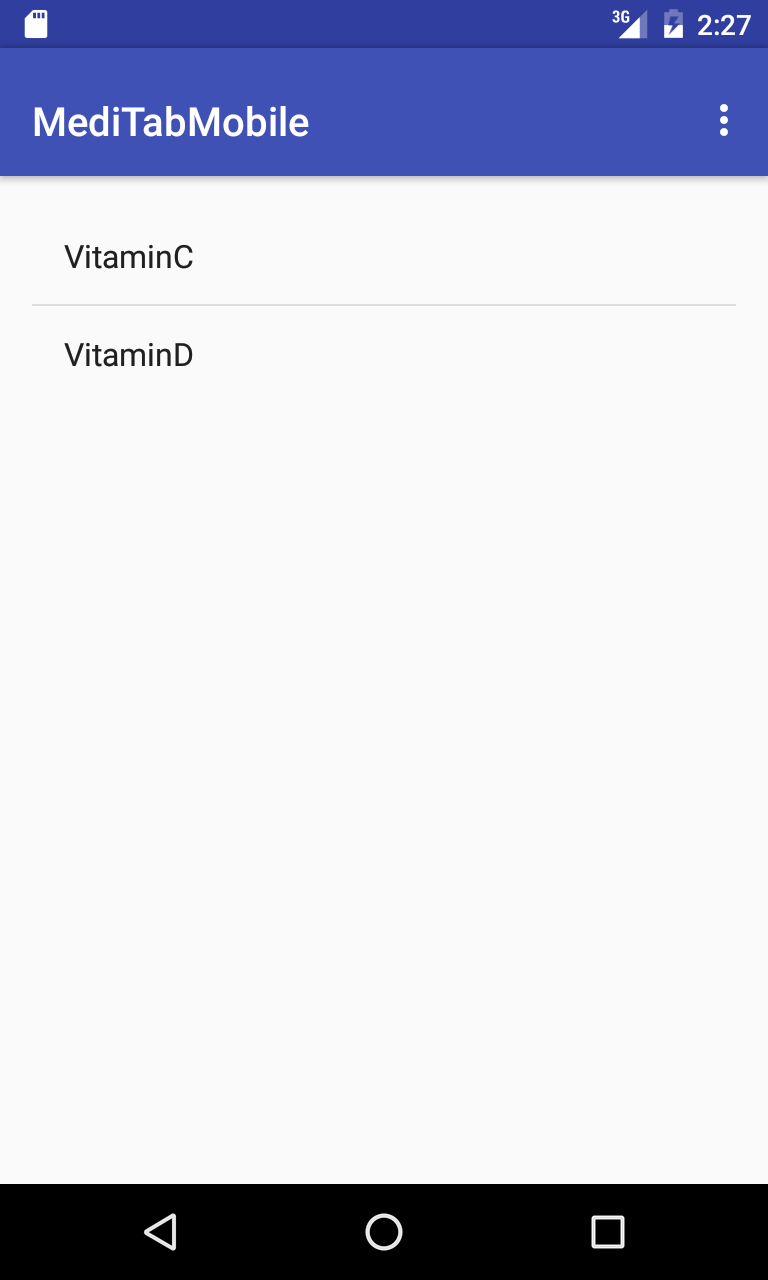
\includegraphics[width=0.4\textwidth]{img/medikace.eps}
	\caption{Medikace}
  \label{medikace}
\end{figure}

Druhý fragment zobrazuje bilanci tekutin daného pacienta, příjem a výdej, v textovém poli (obr. \ref{bilance}).

\begin{figure}[H]
	\centering
	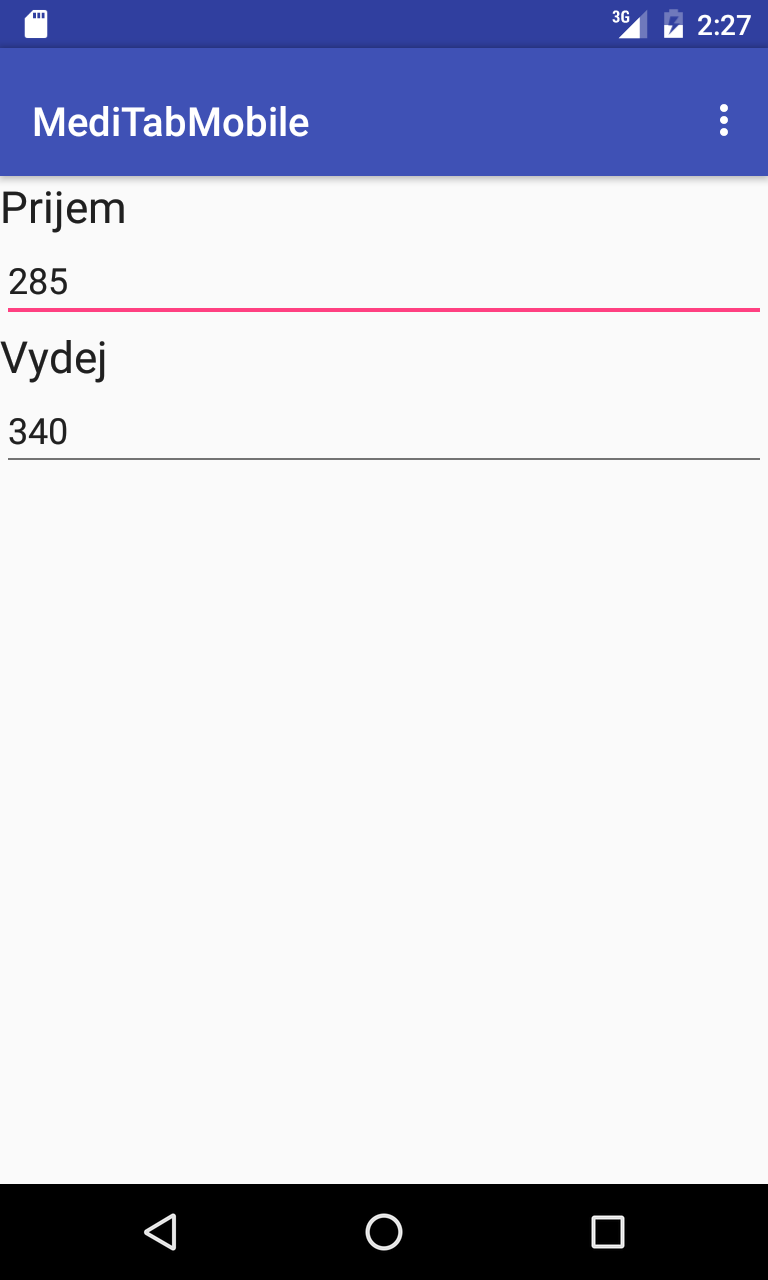
\includegraphics[width=0.4\textwidth]{img/bilance.eps}
	\caption{Bilance tekutin}
  \label{bilance}
\end{figure}


\section{Ordinace}

V ListView je 24 ordinací vybraného léku (obr. \ref{ordinace}). Zobrazuje se datum, množství a stav předepsání. Seznam ordinací  a layout (simple\_list\_item\_2) pro ListView zprostředkovává ArrayAdapter z pole ordinací. Kliknutím na ordinaci se provede její podání (podat lze pouze předepsanou ordinaci - stav 'O').

\begin{figure}[H]
	\centering
	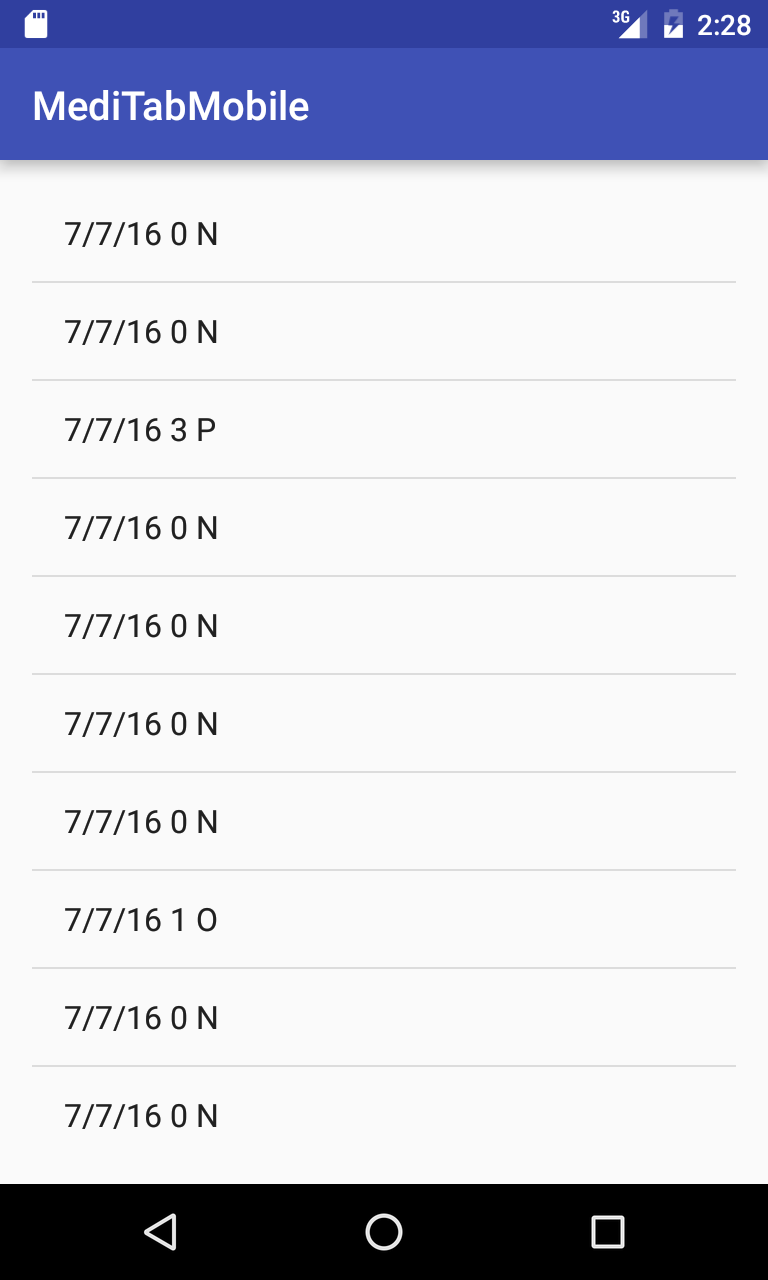
\includegraphics[width=0.4\textwidth]{img/ordinace.eps}
	\caption{Ordinace}
  \label{ordinace}
\end{figure}



%%%%%%%%%%%%%%%%%%%%%%%%%%%%%%%%%%%%%%%%%%%%%%%%%%%%%%%%%%%%%%%%%%%%%%%%%%%%%%%%%%%%%%%%%%%%%%%%%%%%



\chapter{Závěr}

Veškerá data nemocnice jsou v Oracle databázi. Pro budoucí reálné využití aplikace se musí implementovat práce s touto databází.

Dále je v plánu rozšířit funkčnost aplikace, aby rozsahem odpovídala aplikaci MediTab. Celý vývoj se pravděpodobně přesune na platformu Xamarin s využítím jazyku Java a C\#.